%% 该模板修改自《计算机学报》latex 模板
%% 主要是将双栏改成单栏,去掉了部分计算机学报标识;
%% 源文件自:https://www.overleaf.com/latex/templates/latextemplet-cjc-xelatex/ybmmymncrrmw
%% 
%%
%% This is file `CjC_template_tex.tex',
%% is modified by Zhi Wang (zhiwang@ieee.org) based on the template 
%% provided by Chinese Journal of Computers (http://cjc.ict.ac.cn/).
%%
%% This version is capable with Overleaf (XeLaTeX).
%%
%% Update date: 2023/03/10
%% -------------------------------------------------------------------
%% Copyright (C) 2016--2023 
%% -------------------------------------------------------------------
%% This file may be distributed and/or modified under the
%% conditions of the LaTeX Project Public License, either version 1.3c
%% of this license or (at your option) any later version.
%% The latest version of this license is in
%%    https://www.latex-project.org/lppl.txt
%% and version 1.3c or later is part of all distributions of LaTeX
%% version 2008 or later.
%% -------------------------------------------------------------------

\documentclass[10.5pt,compsoc,UTF8]{CjC}
\usepackage{CTEX}
\usepackage{graphicx}
\usepackage{footmisc}
\usepackage{subfigure}
\usepackage{url}
\usepackage{multirow}
\usepackage{multicol}
\usepackage[noadjust]{cite}
\usepackage{amsmath,amsthm}
\usepackage{amssymb,amsfonts}
\usepackage{booktabs}
\usepackage{color}
\usepackage{ccaption}
\usepackage{booktabs}
\usepackage{float}
\usepackage{fancyhdr}
\usepackage{caption}
\usepackage{xcolor,stfloats}
\usepackage{comment}
\setcounter{page}{1}
\graphicspath{{figures/}}
\usepackage{cuted}%flushend,
\usepackage{captionhack}
\usepackage{epstopdf}
\usepackage{gbt7714}

%===============================%

\headevenname{\mbox{\quad} \hfill  \mbox{\zihao{-5}{ \hfill 机器学习  } \hspace {50mm} \mbox{2024 年 5 月}}}%
\headoddname{韩海宇,左益州 \hfill 传统图像分类方法在FashionMNIST数据集上的实验比较}%

%footnote use of *
\renewcommand{\thefootnote}{\fnsymbol{footnote}}
\setcounter{footnote}{0}
\renewcommand\footnotelayout{\zihao{5-}}

\newtheoremstyle{mystyle}{0pt}{0pt}{\normalfont}{1em}{\bf}{}{1em}{}
\theoremstyle{mystyle}
\renewcommand\figurename{figure~}
\renewcommand{\thesubfigure}{(\alph{subfigure})}
\newcommand{\upcite}[1]{\textsuperscript{\cite{#1}}}
\renewcommand{\labelenumi}{(\arabic{enumi})}
\newcommand{\tabincell}[2]{\begin{tabular}{@{}#1@{}}#2\end{tabular}}
\newcommand{\abc}{\color{white}\vrule width 2pt}
\renewcommand{\bibsection}{}
\makeatletter
\renewcommand{\@biblabel}[1]{[#1]\hfill}
\makeatother
\setlength\parindent{2em}
%\renewcommand{\hth}{\begin{CJK*}{UTF8}{gbsn}}
%\renewcommand{\htss}{\begin{CJK*}{UTF8}{gbsn}}


\begin{document}

\hyphenpenalty=50000
\makeatletter
\newcommand\mysmall{\@setfontsize\mysmall{7}{9.5}}
\newenvironment{tablehere}
  {\def\@captype{table}}

\let\temp\footnote
\renewcommand \footnote[1]{\temp{\zihao{-5}#1}}


\thispagestyle{plain}%
\thispagestyle{empty}%
\pagestyle{CjCheadings}

% \begin{table*}[!t]
\vspace {-13mm}


\onecolumn
\zihao{5-}\noindent 韩海宇,左益州\hfill 机器学习\hfill 2024 年 5 月\\
\noindent\rule[0.25\baselineskip]{\textwidth}{1pt}

% \onecolumn
% \zihao{5-}\noindent 第??卷\quad 第?期 \hfill 计\quad 算\quad 机\quad 学\quad 报\hfill Vol. ??  No. ?\\
% \zihao{5-}
% 20??年?月 \hfill CHINESE JOURNAL OF COMPUTERS \hfill ???. 20??\\ 
% \noindent\rule[0.25\baselineskip]{\textwidth}{1pt}

{
\centering
\vspace {11mm}
{\zihao{2} \heiti 传统图像分类方法在FashionMNIST数据集上的实验比较 }

\vskip 5mm

{\zihao{4}\fangsong 韩海宇$^{1)}$\quad  左益州$^{1),}$}

% \footnote{\noindent \zihao{6} 
% % 收稿日期:\quad \quad -\quad -\quad ;最终修改稿收到日期:\quad \quad -\quad -\quad .*投稿时不填写此项*. 本课题得到… …基金中文完整名称(No.项目号)、… …基金中文完整名称(No.项目号)、… … 基金中文完整名称(No.项目号)资助.
% \textsf{作者名1},学号,学位(或目前学历),主要研究领域为*****、****. E-mail: **************.\textsf{作者名2},学号,学位(或目前学历),主要研究领域为*****、****. E-mail: **************. \textsf{作者名3},学号,学位(或目前学历),主要研究领域为*****、****. E-mail: **************.}

\vspace {5mm}

\zihao{5}{$^{1)}$西安电子科技大学杭州研究院}


% \zihao{6}{\textsf{论文定稿后,作者署名、单位无特殊情况不能变更。若变更,须提交签章申请,国家为中国可以不写,省会城市不写省名,其他国家必须写国家名。}}
}

\vskip 5mm

\zihao{5}{
\setlength{\baselineskip}{16pt}\selectfont{
\noindent {\heiti 摘\quad 要\quad }
本次作业旨在探讨传统图像分类方法在FashionMNIST数据集上的应用,并与前馈神经网络进行对比实验。使用手工特征结合SVM算法进行分类任务,分析SVM核函数类型及不同参数设置对分类效果的影响。在训练过程中解决了运行时间长和参数调优的问题。实验结果显示,SVM算法结合像素值特征在测试集上取得了约87.55$\%$的准确率,HOG特征则达到了约84.14$\%$的准确率。多项式核函数的SVM模型准确率高于线性核函数,分别为87.55$\%$和83.70$\%$。与之相比,前馈神经网络在测试集上达到了88.88$\%$的准确率,略优于SVM。实验还发现了一些类别容易混淆的情况,并提出了改进方法。
\par}}
\vspace {5mm}

\zihao{5}{\noindent
{\heiti 关键词 \quad }{传统图像分类;FashionMNIST;手工特征;SVM算法;前馈神经网络;参数调优  }
}
% \zihao{5-}{\heiti 中图法分类号\quad } TP\rm{\quad \quad \quad     }
% {\heiti DOI号:\quad } *投稿时不提供DOI号


\vskip 7mm

\begin{center}
\zihao{3}{ \heiti Experimental Comparison of Traditional Image Classification Methods on the FashionMNIST Dataset}\\
\vspace {5mm}
\zihao{5}{ Han Haiyu$^{1)}$ Zuo Yizhou$^{1)}$ }\\
\vspace {2mm}
\zihao{5-}{{$^{1)}$Hangzhou Research Institute, Xidian University}}


\end{center}

\zihao{5}{
\setlength{\baselineskip}{18pt}\selectfont{
{\bf Abstract}\quad .
\zihao{5}{\noindent This assignment aims to explore the application of traditional image classification methods on the FashionMNIST dataset and compare them with feedforward neural networks. We first use handcrafted features combined with the SVM for the classification task, analyzing the impact of different SVM kernel types and parameter settings on classification performance.  We addressed issues such as long running times and parameter tuning. The experimental results show that the SVM algorithm combined with pixel value features achieved an accuracy of approximately 87.55$\%$ on the test set, while the HOG feature model achieved an accuracy of approximately 84.14$\%$. The polynomial kernel SVM model performed better than the linear kernel, with accuracies of 87.55$\%$ and 83.70$\%$ respectively. The feedforward neural network achieved an accuracy of 88.88$\%$ on the test set, slightly outperforming the SVM. The experiments also identified some categories that are prone to confusion and proposed improvement methods. 
\par}}
\vspace {5mm}

{{\bf Keywords}\quad Traditional image classification; FashionMNIST; handcrafted features; SVM algorithm; feedforward neural network; parameter tuning\par}}



%%%%%%%%%%%%%%%%%%%%%%%%%%%%%%%%%%%%%%
\zihao{5}
\vskip 10mm
% \begin{multicols}{1}


%%%%%%%%%%%%%%%%%%%%%%%%%%%%%%%%%%%%%%%%%%
%%%%%%%%%%%%%%%%%%%%%%%%%%%%%%%%%%%%%%%%%%


\section{\heiti 概述}

\subsection{Fashion-MNIST}
\textbf{来源:}论文Fashion-MNIST: a Novel Image Dataset for Benchmarking Machine Learning Algorithms

\textbf{制作方法:}最原始图片是背景为浅灰色的,分辨率为762*1000的jepg图片。然后经过resampled 到 51*73 的彩色图片。然后依次经过7个步骤,最终得到28*28的灰度图。

1. 将输入转换为png图像

2. 修剪任何与边角像素颜色相近的边缘。“接近度”是由RGB空间中最大可能强度的5%以内的距离来定义的。

3. 对像素进行采样,将图像最长边缘的大小调整为28,即跳过一些行和列。

4. 使用半径和标准差为1.0的高斯算子锐化像素,轮廓附近效果越来越好。

5. 将最短的边延长到28,并将图像放在画布的中心。

6. 消去图像的强度。

7. 将图像转换为8位灰度像素

\textbf{类别:}Fashion-MNIST不再是抽象符号,而是更加具象化的人类必需品:服装,共10大类,分别是:t-shirt(T恤),trouser(牛仔裤),pullover(套衫),dress(裙子),coat(外套),sandal(凉鞋),shirt(衬衫),sneaker(运动鞋),bag(包),ankle boot(短靴)。

\begin{figure}[h] % [h]表示图片插入位置在当前位置
    \centering % 图片居中
    \includegraphics[width=0.5\textwidth]{图片2.png} % 指定图片宽度为当前文本宽度的一半    
    \caption{Fashion-MNIST数据集缩略图} % 添加图片标题
\end{figure}

\subsection{灰度图}
灰度图像避免了彩色带来的复杂性。放大图片中的某一小部分,会发现它是一个二维网络值,亦被称之为具有宽度和高度的数组(单个颜色强度很小的单位)。

这个网格中每个像素颜色都有一个对应的数值,每个像素的值范围是0-255。0 表示黑色,255 表示白色,我们可以通过定位像素网格的横纵坐标来获取某一特定位置的像素值。

\begin{figure}[h] % [h]表示图片插入位置在当前位置
    \centering % 图片居中
    \includegraphics[width=0.5\textwidth]{图片b.png} % 指定图片宽度为当前文本宽度的一半    
    \caption{灰度图} % 添加图片标题
\end{figure}

\subsection{SVM算法}
\textbf{线性可分:}在二维空间上,两类点被一条直线完全分开叫做线性可分,可以推广至n维,三维空间对应二维平面分割,多维空间对应超平面分割。

\begin{figure}[h] % [h]表示图片插入位置在当前位置
    \centering % 图片居中
    \includegraphics[width=0.5\textwidth]{图片f.png} % 指定图片宽度为当前文本宽度的一半    
    \caption{线性可分} % 添加图片标题
\end{figure}

\textbf{最大间隔超平面:}以最大间隔把两类样本分开的最佳超平面,使分类更准确,具体要求:

两类样本分别分割在该超平面的两侧;

两侧距离超平面最近的样本点到超平面的距离被最大化;

\textbf{支持向量:}样本中距离超平面最近的一些点。



\textbf{硬间隔和软间隔:}当两组数据是完全线性可分,我们可以找出一个决策边界使得训练集上的分类误差为0,这两种数据就被称为是存在”硬间隔“的,即考虑所有数据点,包括异常点。当两组数据几乎是完全线性可分的,但决策边界在训练集上存在较小的训练误差,这两种数据就被称为是存在“软间隔”,即通过一定规则忽略异常点,考虑针对大多数点的分割。

\begin{figure}[h] % [h]表示图片插入位置在当前位置
    \centering % 图片居中
    \includegraphics[width=0.5\textwidth]{图片h.png} % 指定图片宽度为当前文本宽度的一半    
    \caption{硬软间隔} % 添加图片标题
\end{figure}

\textbf{核函数:}一个从低维空间到高维空间的映射,而这个映射可以把低维空间中线性不可分的两类点变成线性可分的。下图所示的两类数据在二维平面中,这样的数据本身就是线性不可分的,此时我们就要思考该如何把这两类数据分开,当我们通过一定的映射,将二维数据升为三维数据,就成为线性可分的数据

\textbf{线性核和多项式核:}

1)这两种核的作用也是首先在属性空间中找到一些点,把这些点当做base,核函数的作用就是找与该点距离和角度满足某种关系的样本点。

2)样本点与该点的夹角近乎垂直时,两个样本的欧式长度必须非常长才能保证满足线性核函数大于0;而当样本点与base点的方向相同时,长度就不必很长;而当方向相反时,核函数值就是负的,被判为反类。即,它在空间上划分出一个梭形,按照梭形来进行正反类划分。

\begin{figure}[h] % [h]表示图片插入位置在当前位置
    \centering % 图片居中
    \includegraphics[width=0.4\textwidth]{图片i.png} % 指定图片宽度为当前文本宽度的一半    
    \caption{二维线性不可分} % 添加图片标题
\end{figure}

\begin{figure}[h] % [h]表示图片插入位置在当前位置
    \centering % 图片居中
    \includegraphics[width=0.5\textwidth]{图片j.png} % 指定图片宽度为当前文本宽度的一半    
    \caption{升维为线性可分} % 添加图片标题
\end{figure}

\subsection{前馈神经网络}
\textbf{结构:}输入层,即输入x的那一层;输出层,即输出y的那一层;隐藏层,输入层和输出层之间不管隔了多少层都叫隐藏层。

\begin{figure}[h] % [h]表示图片插入位置在当前位置
    \centering % 图片居中
    \includegraphics[width=0.8\textwidth]{图片k.png} % 指定图片宽度为当前文本宽度的一半    
    \caption{神经网络} % 添加图片标题
\end{figure}

\textbf{激活函数:}假设输入特征只有一个特征,那么上图的输出就是个线性函数。你也可以将隐藏层设为多个节点,算出来的输出仍然是关于的线性函数。所以如果激活函数是线性的,神经网络叠再多层也没什么意义,和最基本的线性回归是一模一样的。因此将激活函数应用到隐藏层上,可以增加非线性因素,解决线性模型表达能力不足的缺陷。

\begin{figure}[h] % [h]表示图片插入位置在当前位置
    \centering % 图片居中
    \includegraphics[width=0.5\textwidth]{图片l.png} % 指定图片宽度为当前文本宽度的一半    
    \caption{激活函数} % 添加图片标题
\end{figure}

\textbf{损失函数:}损失函数用于量化模型预测与真实值之间的差异。它是预测值与真实值之间差距的计算方法,并通过深度学习框架(如PyTorch、TensorFlow)进行封装。

\begin{figure}[h] % [h]表示图片插入位置在当前位置
    \centering % 图片居中
    \includegraphics[width=0.5\textwidth]{图片m.png} % 指定图片宽度为当前文本宽度的一半    
    \caption{损失函数} % 添加图片标题
\end{figure}

\textbf{训练过程:}

1)抽取训练样本x和对应的目标y组成数据批量

2)在x上运行网络(这一步被称为前向传播),得到预测值ypred

3)计算网络在这批数据上的损失,用于衡量ypred和y之间的距离

4)计算损失相对于网络参数的梯度(一次反向传播)

5)将参数沿着梯度的反方向移动一点(步长),从而使得这批数据上的损失减小一点,这种方法就是小批量随机梯度下降
\begin{figure}[h] % [h]表示图片插入位置在当前位置
    \centering % 图片居中
    \includegraphics[width=0.5\textwidth]{图片n.png} % 指定图片宽度为当前文本宽度的一半    
    \caption{训练过程} % 添加图片标题
\end{figure}
\section{\heiti 问题}

\subsection{运行时间长}
无论是使用SVM还是前馈神经网络进行训练,当使用完整的训练集(60000张图片)时,训练时间很长,但是也并没有占用很多内存,最终长时间不能生成结果。

\textbf{解决办法一:缩减数据集规模。}首先将训练集切片至10000,再去执行,发现可以在较短时间内生成结果,因此排除代码问题。
\begin{figure}[h] % [h]表示图片插入位置在当前位置
    \centering % 图片居中
    \includegraphics[width=0.8\textwidth]{图片o.png} % 指定图片宽度为当前文本宽度的一半    
    \caption{缩减数据集操作} % 添加图片标题
\end{figure}

\textbf{解决办法二:}标准化处理。归一化或者标准化的目的就是使得预处理的数据被限定在一定的范围内(比如[0,1]或者[-1,1]),从而消除奇异样本数据导致的不良影响。譬如,下面为具有两个特征的样本数据x1、x2、x3、x4、x5、x6,其中x6这个样本的两个特征相对其他样本而言相差比较大,因此,x6认为是奇异样本数据。
\begin{figure}[h] % [h]表示图片插入位置在当前位置
    \centering % 图片居中
    \includegraphics[width=0.8\textwidth]{图片q.png} % 指定图片宽度为当前文本宽度的一半    
    \caption{奇异点} % 添加图片标题
\end{figure}

奇异样本数据的存在会引起训练时间增大,同时也可能导致无法收敛,因此,当存在奇异样本数据时,在进行训练之前需要对预处理数据进行归一化。如果不进行归一化,那么由于特征向量中不同特征的取值相差较大,会导致目标函数变“扁”。这样在进行梯度下降的时候,梯度的方向就会偏离最小值的方向,走很多弯路,即训练时间过长。如果进行归一化以后,目标函数会呈现比较“圆”,这样训练速度大大加快,少走很多弯路。
\begin{figure}[h] % [h]表示图片插入位置在当前位置
    \centering % 图片居中
    \includegraphics[width=0.5\textwidth]{图片s.png} % 指定图片宽度为当前文本宽度的一半    
    \caption{归一化后的收敛路径} % 添加图片标题
\end{figure}

\subsection{参数调优}
神经网络可以设置层数,节点数,激活函数,求解器等多个参数,不同组合下其训练的效果并不相同,如果和SVM算法进行对比的话,理论上应该选取具有最优参数的神经网络与SVM进行对比,如何实现?

\textbf{解决办法:}网格搜索。网格搜索的基本思想是通过穷举搜索指定参数的所有可能组合,以找到在验证集上表现最佳的参数集。对于神经网络,常见的超参数包括:隐藏层大小,学习率,激活函数,优化算法最大迭代次数

\textbf{工作原理:}

定义参数网格:确定需要优化的超参数及其可能的取值范围。

生成参数组合:生成所有可能的参数组合。

评估模型性能:对于每一组参数组合,使用交叉验证评估模型性能。

选择最佳参数组合:根据交叉验证的平均性能指标,选择表现最好的参数组合。
\begin{figure}[h] % [h]表示图片插入位置在当前位置
    \centering % 图片居中
    \includegraphics[width=0.7\textwidth]{图片t.png} % 指定图片宽度为当前文本宽度的一半    
    \caption{网格搜索操作} % 添加图片标题
\end{figure}

\section{\heiti 训练及验证结果}

\subsection{准确度分析}
不同的求解器类型和参数设置,其对应的准确度如下:
\begin{table}[htbp]
\centering {\heiti 表1\quad 准确度分析}
% \caption{表说明 *表说明采用黑体*}
\vspace {-2.5mm}
\begin{center}
\begin{tabular}{l     l}
\toprule
类型&准确度 \\
\hline
SVM+HOG+linear&0.8052
 \\
SVM+HOG+poly&0.8414
 \\
SVM+像素值+linear&0.8370
 \\
SVM+像素值+poly&\textbf{0.8755}
 \\
 前馈神经网络&\textbf{0.8888}
 \\
\bottomrule
\end{tabular}
\label{tab1}
\end{center}
\end{table}

\textbf{结论一:像素值特征的效果优于HOG特征},主要原因可能有以下几点:

1、简单图像结构:Fashion-MNIST的数据集包含的图像相对简单,每个图像是28x28像素的灰度图,表示10类不同的服饰。这些图像中的对象通常是居中的,并且背景简单。因此,直接使用像素值作为特征就已经包含了足够的区分信息。

2、低分辨率:Fashion-MNIST图像的低分辨率(28x28像素)意味着像素值特征的维度是784,尽管维度较高,但在当前的计算能力下仍然可以有效处理。而HOG特征在提取过程中可能丢失一些关键细节,尤其是对于低分辨率图像。

3、HOG特征的维度通常比原始像素值要低。尽管这在某些情况下有助于减少计算复杂度和过拟合,但对于Fashion-MNIST这样简单的任务,较高维度的像素值特征反而可能提供更多的区分信息,有助于分类器的性能。

4、不同的特征类型可能需要不同的超参数设置。例如,HOG特征提取后的数据可能需要不同的SVM参数设置(如C值、gamma值等)来达到最佳性能。如果没有针对HOG特征进行细致的超参数调整,可能导致其性能不如直接使用像素值。

\textbf{结论二:多项式核函数的效果优于线性核函数},主要原因可能有以下几点:

1. 数据的非线性可分性:Fashion-MNIST数据集中的样本通常不是线性可分的。线性核函数假设数据在高维空间中是线性可分的,这对某些复杂的数据集来说是一个限制。相比之下,多项式核函数能够映射数据到更高维的多项式特征空间,使得在这个空间中更容易找到一个超平面来分离不同类别的样本

2. 多项式核函数的灵活性:多项式核函数通过参数调整(如多项式的度数)可以灵活地控制模型的复杂度。较低度数的多项式核可以捕捉到较简单的模式,而较高度数的多项式核则可以捕捉到更复杂的模式。这种灵活性使得多项式核函数在处理复杂数据时比线性核函数更有优势。

3. 适应复杂模式:Fashion-MNIST数据集中的服饰类别(如T恤、裤子、鞋子等)具有不同的形状和结构,这些模式往往是非线性的。多项式核函数能够更好地适应这些复杂的模式,而线性核函数则可能不足以捕捉到这些模式的所有细节。

\textbf{结论三:前馈神经网络效果优于svm}。其原因可能是:

1. 非线性特征学习能力:FNN能够通过多层结构自动学习输入数据的非线性特征。每一层都可以对前一层的输出进行复杂的非线性变换,从而捕捉到数据的复杂模式。SVM尽管使用核函数(如高斯核、RBF核)可以让SVM处理非线性数据,但它的非线性学习能力有限,尤其是在高维数据集上,可能无法捕捉到数据的复杂模式。

2. 适应性:前馈神经网络FNN可以通过改变网络结构(如增加层数和神经元数量)来适应不同的任务和数据集。它的灵活性使其在处理各种类型的数据时具有优势。尽管SVM的核函数可以调整以适应不同的任务,但其整体结构相对固定,缺乏灵活性。

3.处理大规模数据:FNN在处理大规模数据时,利用并行计算和GPU加速可以更有效地训练模型。它能够处理大量的输入数据并从中学习复杂的模式。SVM在处理大规模数据时,训练时间和内存需求都会急剧增加,尤其是使用复杂的核函数时,这可能成为瓶颈。

4. 泛化能力:FNN通过正则化技术(如Dropout、L2正则化)和早停(Early Stopping)等方法,可以有效地防止过拟合,提高泛化能力。SVM的泛化能力依赖于核函数的选择和参数调优,但在一些复杂数据集上可能不如FNN。
\subsection{混淆矩阵分析}
综合比对各种求解器的结果,观察其混淆矩阵,发现尽管在数值上存在差异,但在分布规律上是一致的,因此在这里提供一个组别的混淆矩阵可视化图像进行分析。
\begin{figure}[h] % [h]表示图片插入位置在当前位置
    \centering % 图片居中
    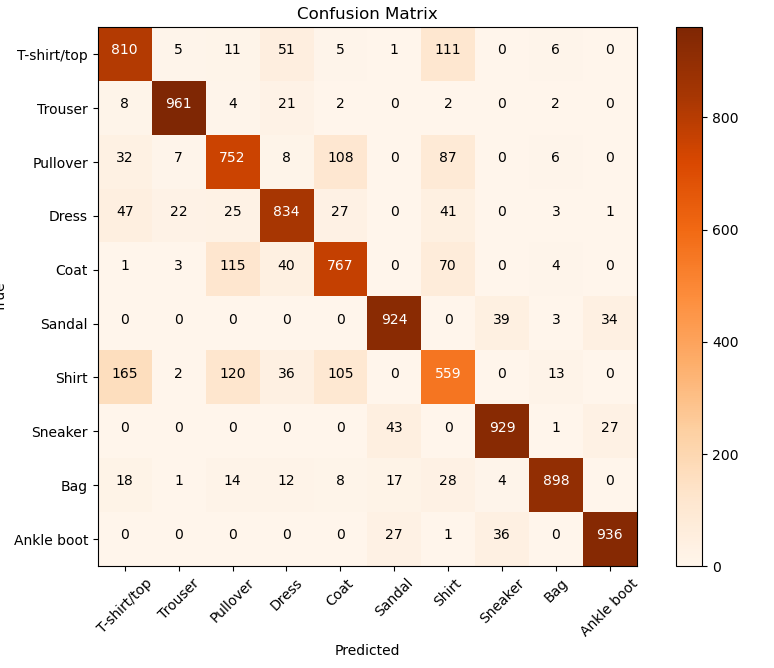
\includegraphics[width=0.7\textwidth]{图片u.png} % 指定图片宽度为当前文本宽度的一半    
    \caption{混淆矩阵可视化} % 添加图片标题
\end{figure}

\textbf{准确率和召回率:}每个类别的准确率表示正确分类该类别的比例。通过观察分类报告中的准确率,可以确定哪些类别的分类效果较好,哪些较差。每个类别的召回率表示该类别中被正确分类的样本比例。低召回率表明模型对该类别的识别能力较差。

\textbf{类别间混淆:}T-shirt/top 和 Shirt:这两个类别容易混淆,因为它们在视觉上比较相似。混淆矩阵中会显示 T-shirt/top 和 Shirt 之间的误分类数量。

Pullover 和 Coat:这两个类别也可能因为形状和外观的相似而被误分类。Sneaker 和 Ankle boot:这两个类别同为鞋类,有可能在某些角度或特定情况下被误分类。

\textbf{改进:}可以增加这些容易混淆类别的样本数量,以提供更多的训练数据。提高图像的分辨率或使用更多的预处理技术(如数据增强),以帮助模型更好地区分不同类别。尝试不同的特征提取方法(如更高级的HOG参数,或使用深度学习方法自动提取特征)来提高分类性能。


\subsection{参考文献}
引用文献1~\cite{DU2024151828},文献2~\cite{WAN2024104773},文献3-5~\cite{HAN2023107839,YUAN2021759,ZHANG2024}。





\vspace {10mm}
\centerline
{\zihao{5}\textsf{参~考~文~献}}
\zihao{5-} \addtolength{\itemsep}{-1em}
\vspace {1.5mm}
\bibliographystyle{gbt7714-numerical}
\bibliography{ref.bib}


% \begin{thebibliography}{99}
% \zihao{5-} \addtolength{\itemsep}{-1em}
% \vspace {1.5mm}

% \bibitem[1]{1}
% 网上的文献(举例:The Cooperative
% Association for Internet Data Analysis(CAIDA),http://www.caida.org/data
% 2010,7,18) \textbf{*请采用脚注放于正文出现处,每页的脚注从1开始编序号*}\footnote{The Cooperative Association for Internet Data
% Analysis (CAIDA), http://www.caida.org/data 2010, 7, 18}

% \bibitem[2]{2} 中文的参考文献需给出中英文对照。形式如[3]。

% \bibitem[3]{3} Zhou Yong-Bin, Feng Deng-Guo. Design and analysis of cryptographic
% protocols for RFID. Chinese Journal of Computers, 2006, 29(4): 581-589 (in
% Chinese) \newline
% (周永彬, 冯登国. RFID安全协议的设计与分析. 计算机学报, 2006, 29(4): 581-589)

% \bibitem[4]{4} 期刊、会议、书籍名称不能用缩写。

% \bibitem[5]{5} 作者(外国人姓在前,名在后可缩写, 后同).
% 题目(英文题目第一字母大写,其它均小写):副标题(如果有). 刊名(全称), 年,
% 卷(期): 页码 \textbf{*期刊论文格式*}

% \bibitem[6]{6}作者.
% 文章题目(英文题目第1字母大写,其它均小写):副标题(如果有)//Proceedings of
% the {\ldots} (会议名称). 会议召开城市, 会议召开城市所在国家, 年: 页码
% \textbf{*会议论文集论文格式*}

% \bibitem[7]{7}作者. 文章题目(英文题目第一字母大写, 其它均小写):
% 副标题(如果有)//编者. 文集标题. 出版地: 出版社, 出版年: 页码
% \textbf{*文集格式*}

% \bibitem[8]{8}作者. 书名: 副标题(如果有). 版次(初版不写). 出版社地点: 出版社,
% 出版年 \textbf{*书籍格式*}

% \bibitem[9]{9}作者. 文章题目[博士学位论文/硕士学位论文]. 单位名称,单位地点, 年
% \textbf{*学位论文格式*}

% \bibitem[10]{10}作者. 文章题目(英文题目第一字母大写,其它均小写). 单位地点: 单位,
% 技术报告: 报告编号, 年 \textbf{*技术报告*}

% \bibitem[11]{11}专利拥有人. 专利名称,专利授权国家,专利授权日期
% \textbf{*技术专利*}

% \end{thebibliography}
% \end{multicols}

% \newpage


% \end{multicols}





%%%%%%%%%%%%%%%%%%%%%%%%%%%%%%%%%%%
%%%%%%%%%%%%%%%%%%%%%%%%%%%%%%%%%%%5




% \begin{multicols}{1}
% \zihao{5}
% \noindent \textbf{Background}

% \zihao{5-}{
% \setlength\parindent{2em}
% *论文背景介绍为\textbf{英文},字体为小5号Times New Roman体*

% 论文后面为400单词左右的英文背景介绍。介绍的内容包括:

% 本文研究的问题属于哪一个领域的什么问题。该类问题目前国际上解决到什么程度。

% 本文将问题解决到什么程度。

% 课题所属的项目。

% 项目的意义。

% 本研究群体以往在这个方向上的研究成果。

% 本文的成果是解决大课题中的哪一部分,如果涉及863$\backslash
% $973以及其项目、基金、研究计划,注意这些项目的英文名称应书写正确。}

% \end{multicols}

\end{document}


